\section{Surfaces}
\label{sec:surfaces}

To explain the drop in performance for SUIM after a budget of 3'500, we computed the true surfaces for all datasets~(\cref{fig:surfaces}). We observed that segmentation performance grows logarithmically for OCT, VOC, and Cityscapes, but not for SUIM after a certain number of class annotations. Since our GP assumes a logarithmic relation between dataset size and performance, this observation is particularly relevant to explain the decline in performance for SUIM. Most notably, and confirming our hypothesis, this decline is not seen with other values of~$\alpha_s$ for this same dataset~(\cref{fig:alpha_results}). Due to the limited dataset size, larger values of $\alpha_s$ constrain the area of the surface that can be reached in our experiments. In the case of SUIM, $\alpha_s = 50$ translates to exploring zones where performance grows logarithmically with dataset size (low data regime).

%\begin{figure}[h]
%\centering
%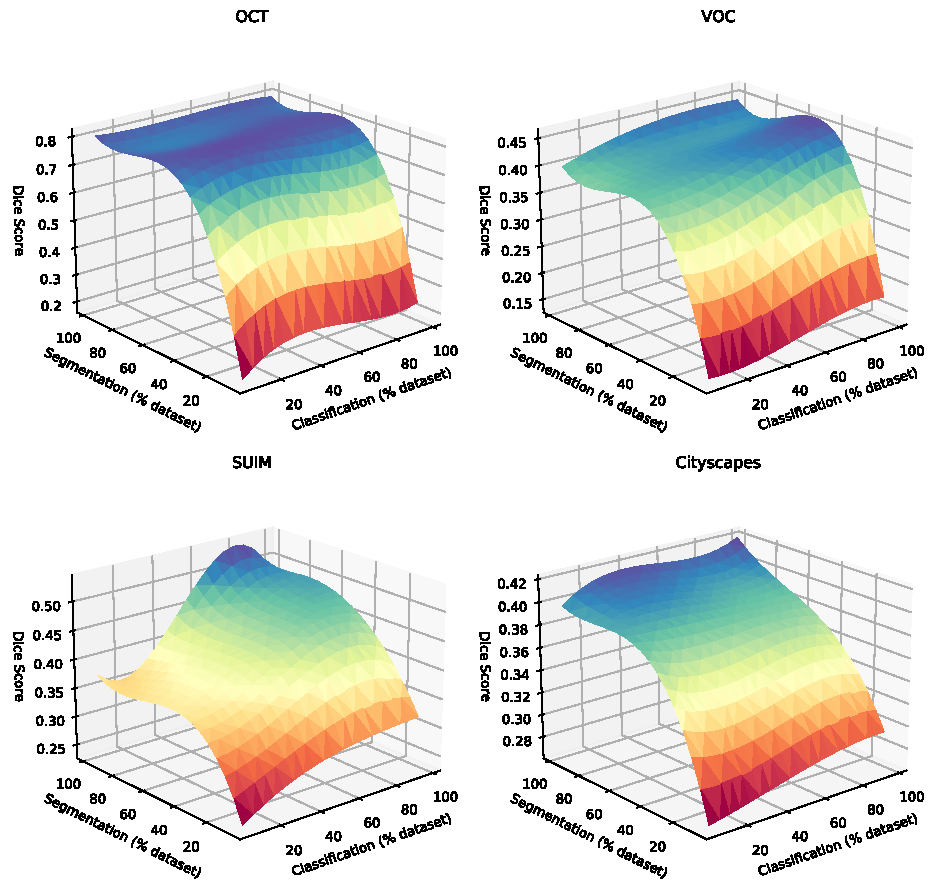
\includegraphics[width=0.8\linewidth]{fullweak/Figures/surface_supp.pdf}
%\caption{Segmentation performance grows logarithmically with training set size on Cityscapes, OCT, and VOC. This trend is not observed in the SUIM dataset. 
%}
%\label{fig:surfaces}
%\end{figure}

\plainwidefig{1}{fullweak/Figures/surface_supp.pdf}{Segmentation performance grows logarithmically with training set size on Cityscapes, OCT, and VOC. This trend is not observed in the SUIM dataset.}{fig:surfaces_fullweak_app}